\chapter{Benutzerschnittstellen}

\section{Kommandozeile}\label{sec:uicmd}

Die Kommandozeilen-Schnittstelle bietet dem Benutzer eine schnelle Möglichkeit Graphdateien beim Programmstart mit zusätzlichen Parametern zu öffnen.
Folgende Parameter werden unterstützt:\\
\subsection{Muss-Argumente}
\begin{tabular}{lp{0.75\linewidth}}
  -layout <layout> & Legt einen Layout-Algorithmus fest, welcher beim Programmstart auf den ersten Graphen angewendet wird.\\
    & Dabei ist <layout> ein Kürzel, das vom jeweiligen Layout-Plugin definiert wird. Das Kürzel wird hinter der Layout-Option in der Menüleiste angezeigt.\\
  -in <datei> & Legt die zu öffnende Graphdatei fest. <datei> ist der relative oder absolute Pfad zu einer Graphdatei. Alternativ kann ``-in'' weggelassen werden, falls der Pfad als letztes Argument angegeben wird.\\
  -type <typeid> & Legt den Typ des Graphen fest. Über den Typ des Graphen wird das Import-Plugin, sowie initiale Darstellungsoptionen festgelegt. Graphtypen können von Plugins definiert werden. (siehe ) %TODO: Referenz Pluginsschnittstellen)
\end{tabular}

\subsection{Kann-Argumente}
\begin{tabular}{lp{0.75\linewidth}}
  -out <datei> & Legt einen Pfad zu einer Datei fest, in welcher der Graph gespeichert werden soll.
  Es wird die in %TODO: Referenz zu Kann Funktion zum speichern von graphen
  beschrieben Funktion ausgeführt.
  Falls angegeben, wird der Layout-Algorithmus auf alle Graphen in der zu öffnenden Datei angewendet, bevor das Speichern beginnt.
  Die \gls{gui} wird nicht gestartet.
\end{tabular}

\section{GUI}\label{sec:uigui}

Die graphische Oberfläche bietet dem Benutzer ein interaktives Interface und eine Anzeige für die gelayouteten Graphen. %TODO: gelayoutet ersetzen

\subsection{Entwürfe}

Bemerkungen zu den folgenden Entwurfsabbildungen: Die Funktionalität weicht in der Implementierung eventuell von der Darstellung hier ab. Die Darstellung dient lediglich einer generellen Übersicht der GUI und ist als solche als Prototyp zu verstehen.

\begin{figure}[ht]
  \centering
  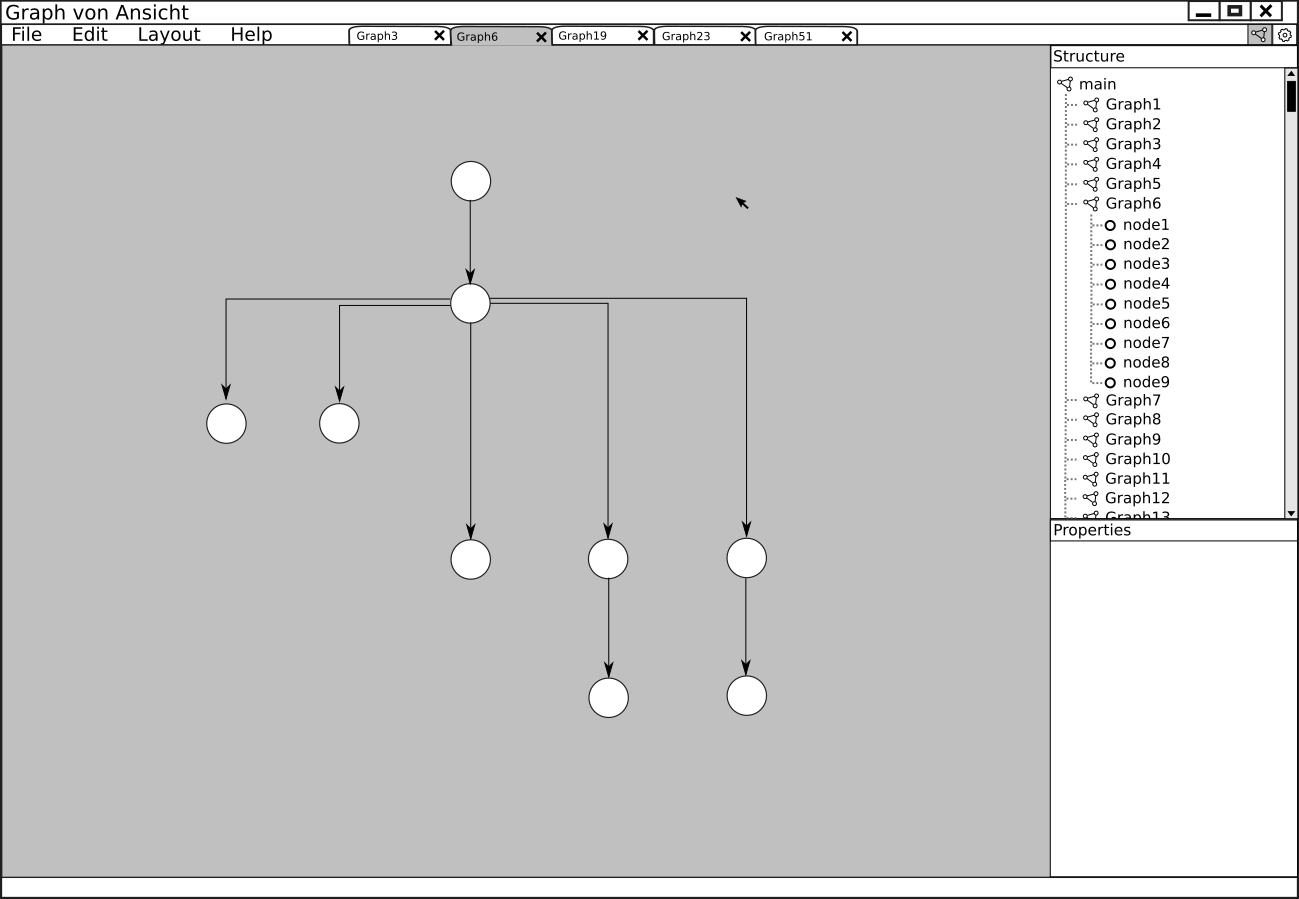
\includegraphics[width=380pt]{resourcen/gui_view_treeview.png}
  \caption{Hauptansicht}
  \label{fig:gui_view_treeview}
\end{figure}

\begin{figure}[ht]
  \centering
  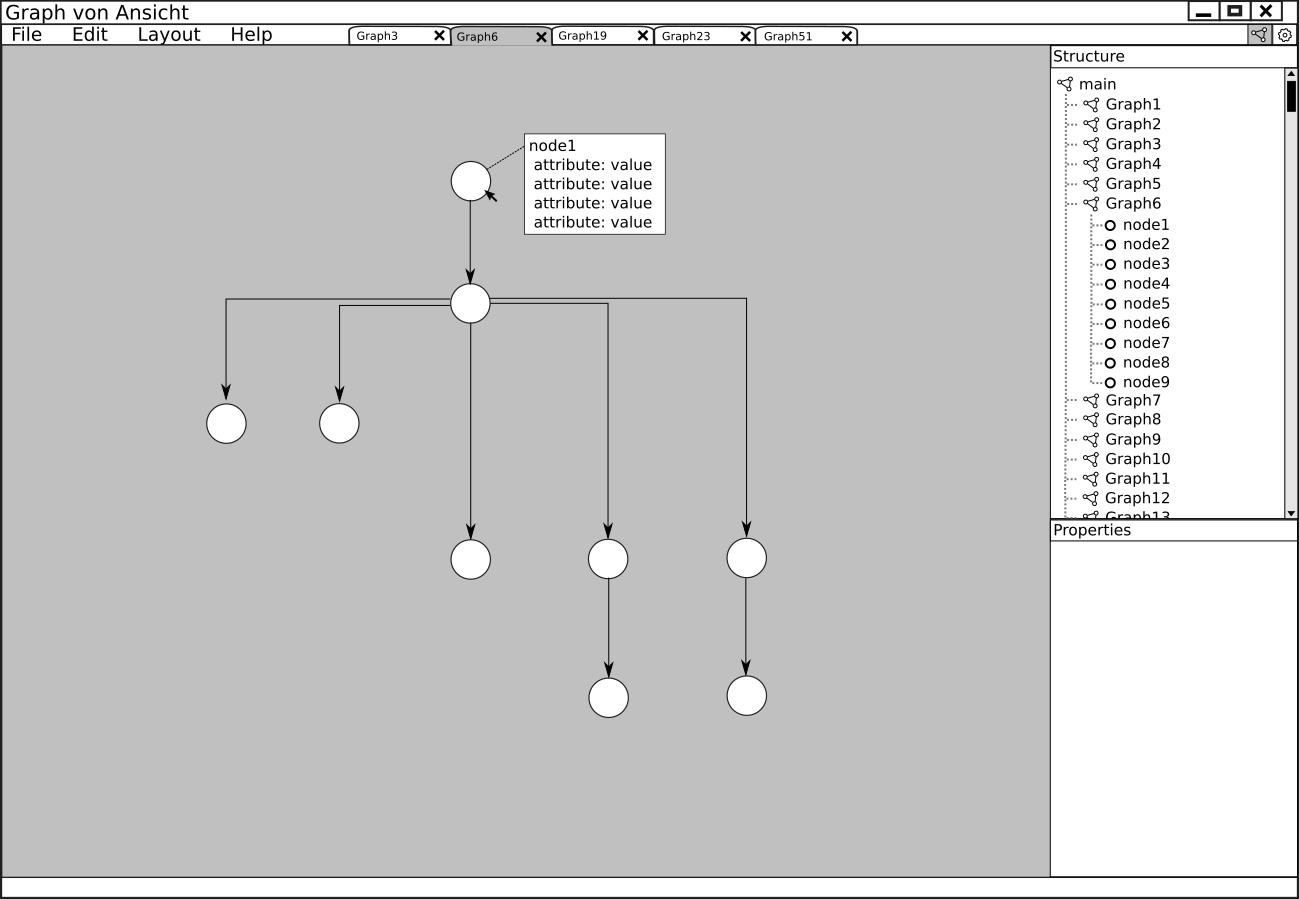
\includegraphics[width=380pt]{resourcen/gui_view_showInfoInView_node.png}
  \caption{Knoteninformation anzeigen}
  \label{fig:gui_view_showInfoInView_node}
\end{figure}

\begin{figure}[ht]
  \centering
  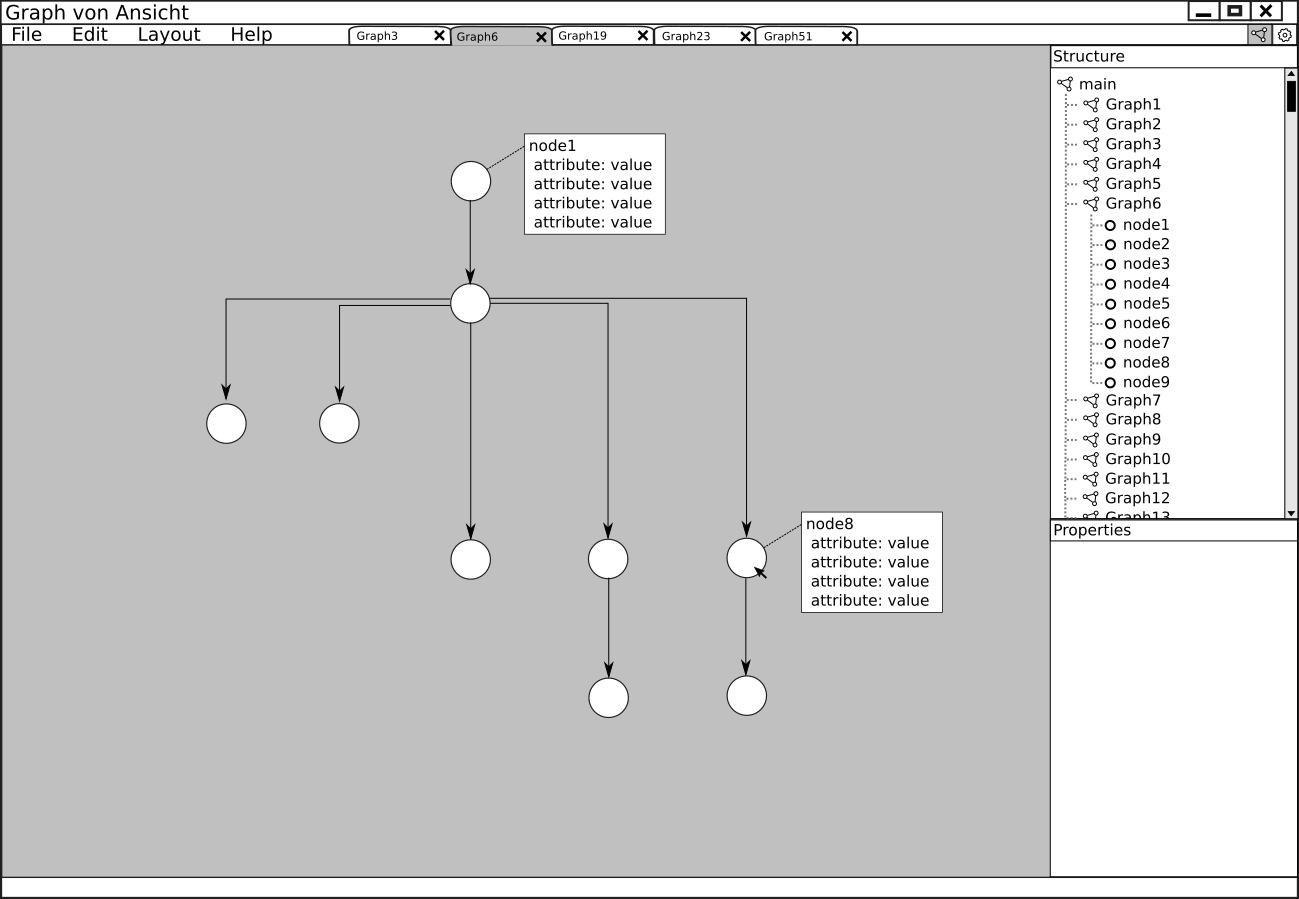
\includegraphics[width=380pt]{resourcen/gui_view_showInfoInView_node_multi.png}
  \caption{Mehrere Knoteninformationen anzeigen}
  \label{fig:gui_view_showInfoInView_node_multi}
\end{figure}

\begin{figure}[ht]
  \centering
  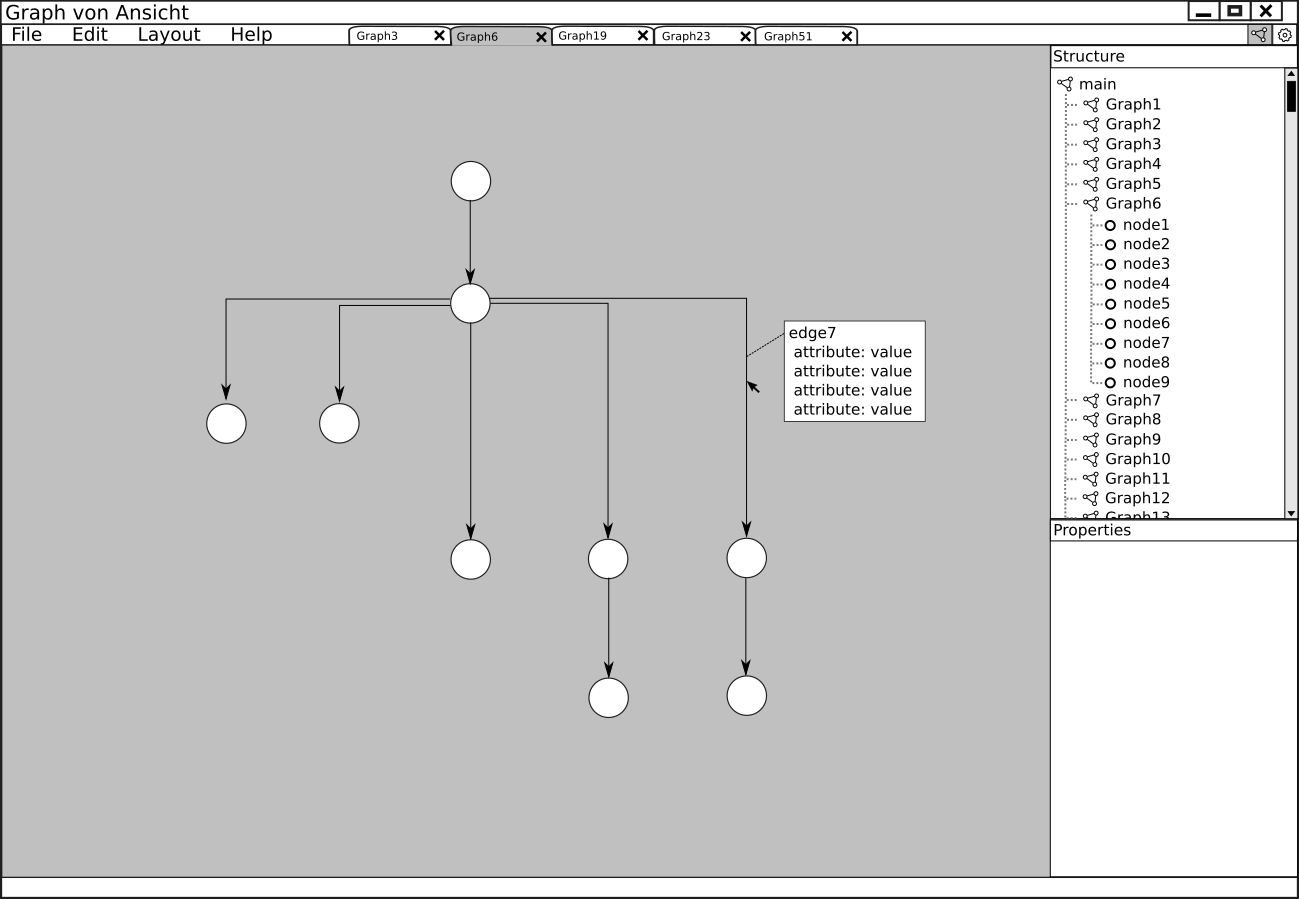
\includegraphics[width=380pt]{resourcen/gui_view_showInfoInView_edge.png}
  \caption{Kanteninformation Anzeigen}
  \label{fig:gui_view_showInfoInView_edge}
\end{figure}

\begin{figure}[ht]
  \centering
  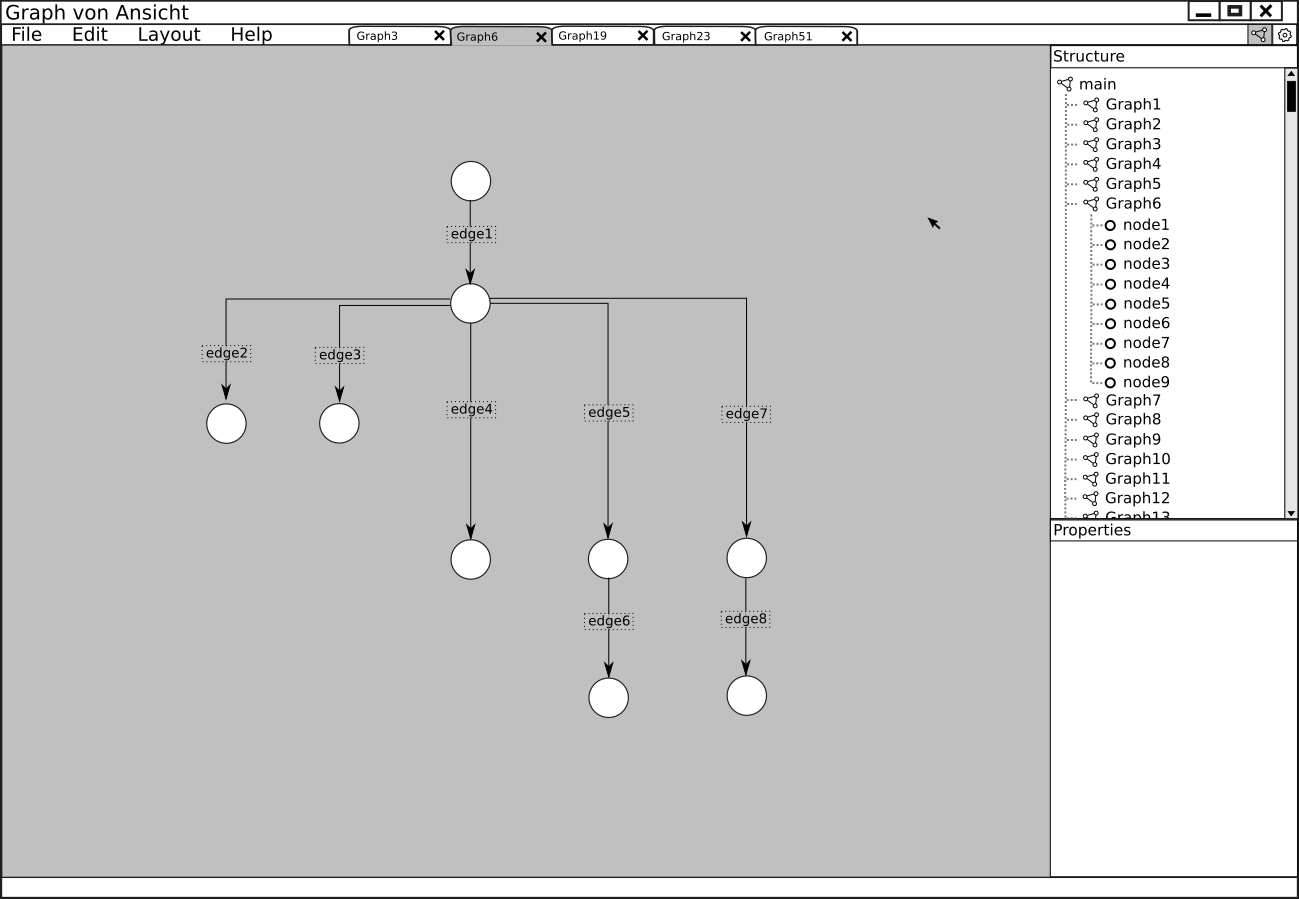
\includegraphics[width=380pt]{resourcen/gui_view_showInfoInView_edge_all.png}
  \caption{Anzeige aller Kantennamen}
  \label{fig:gui_view_showInfoInView_edge_all}
\end{figure}

\begin{figure}[ht]
  \centering
  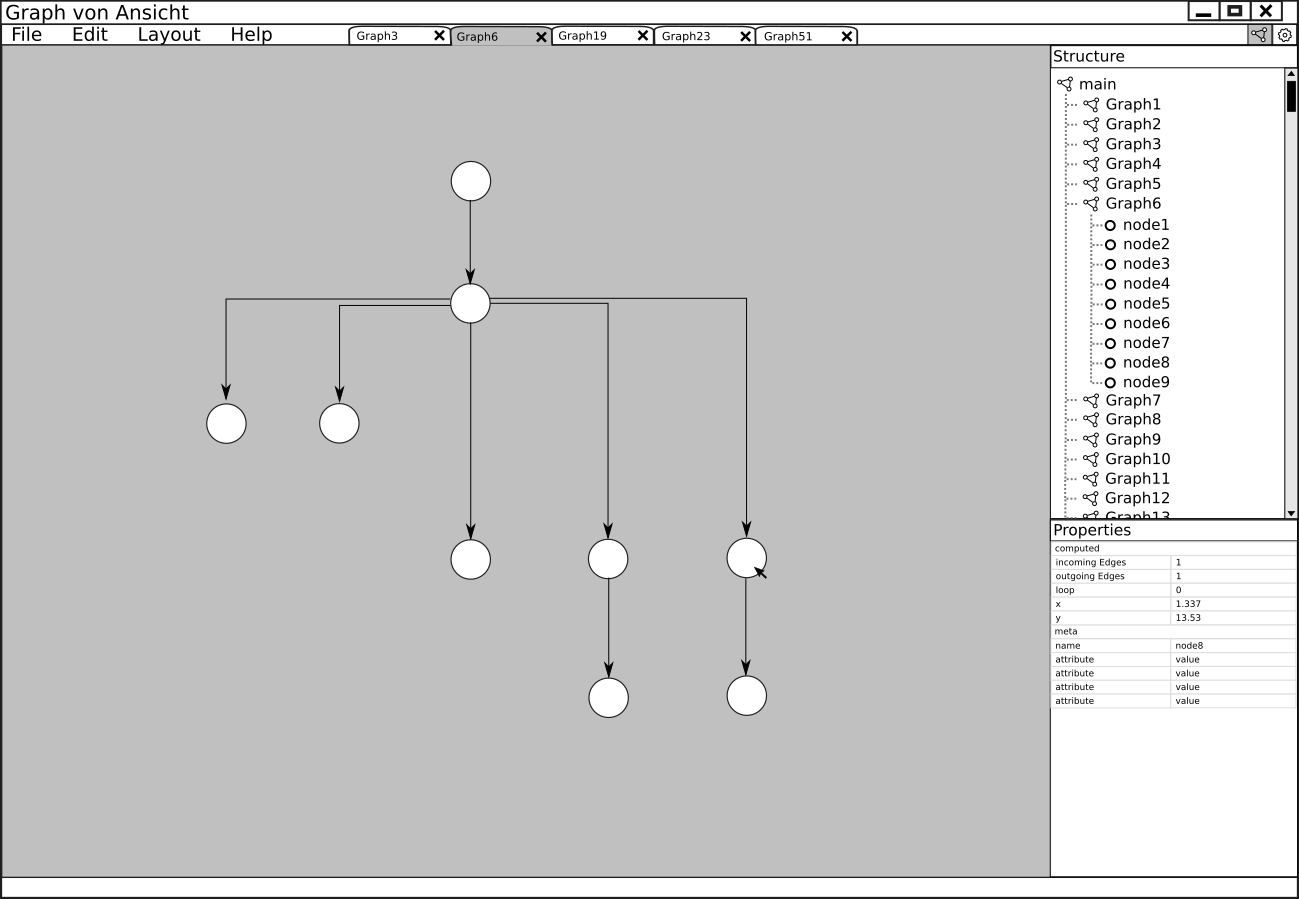
\includegraphics[width=380pt]{resourcen/gui_view_showInfoInProperties_node.png}
  \caption{Eigenschaftenansicht von Knoten}
  \label{fig:gui_view_showInfoInProperties_node}
\end{figure}

\begin{figure}[ht]
  \centering
  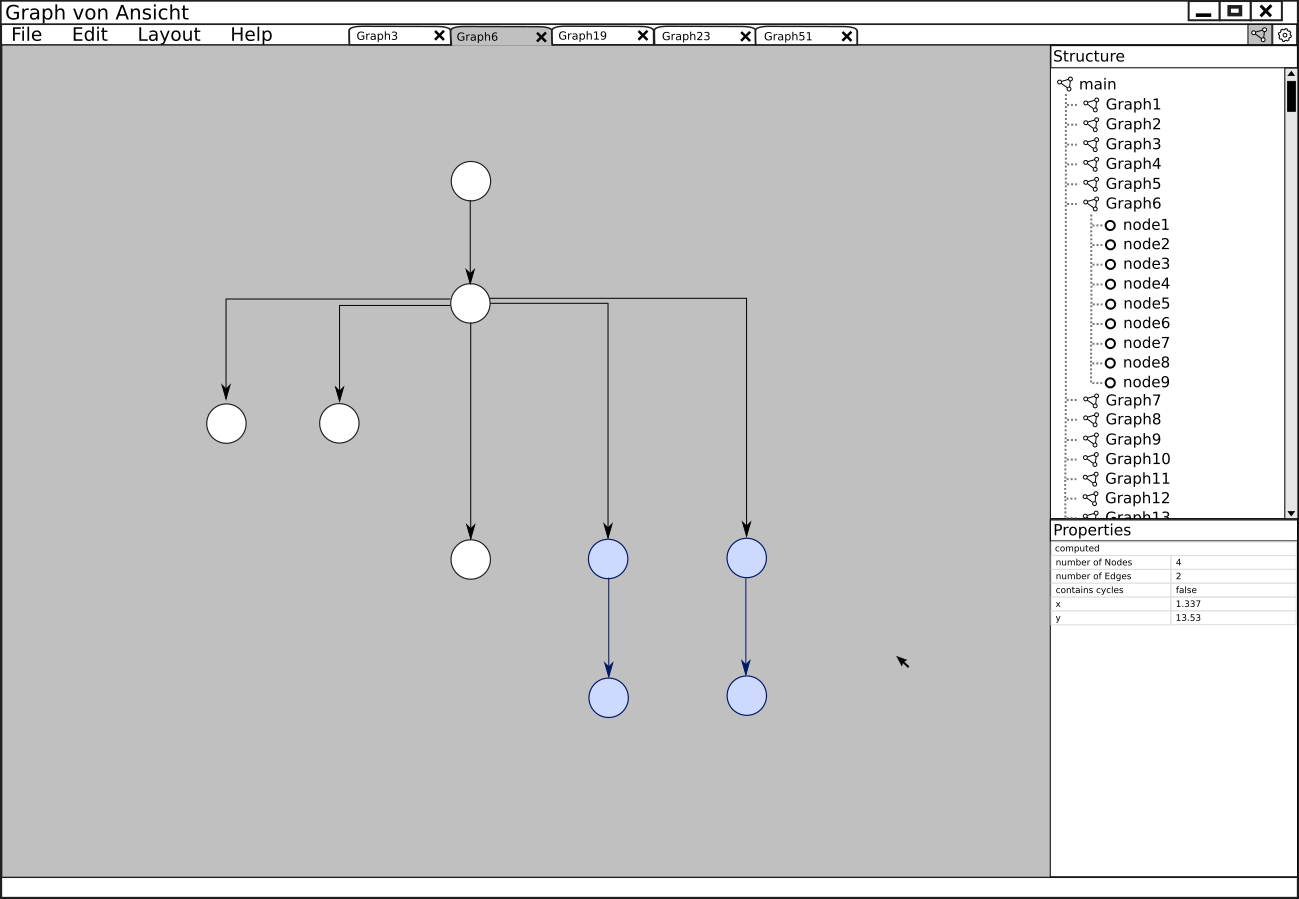
\includegraphics[width=380pt]{resourcen/gui_view_showInfoInProperties_multi.png}
  \caption{Eigenschaftenansicht von mehreren Knoten}
  \label{fig:gui_view_showInfoInProperties_multi}
\end{figure}

\begin{figure}[ht]
  \centering
  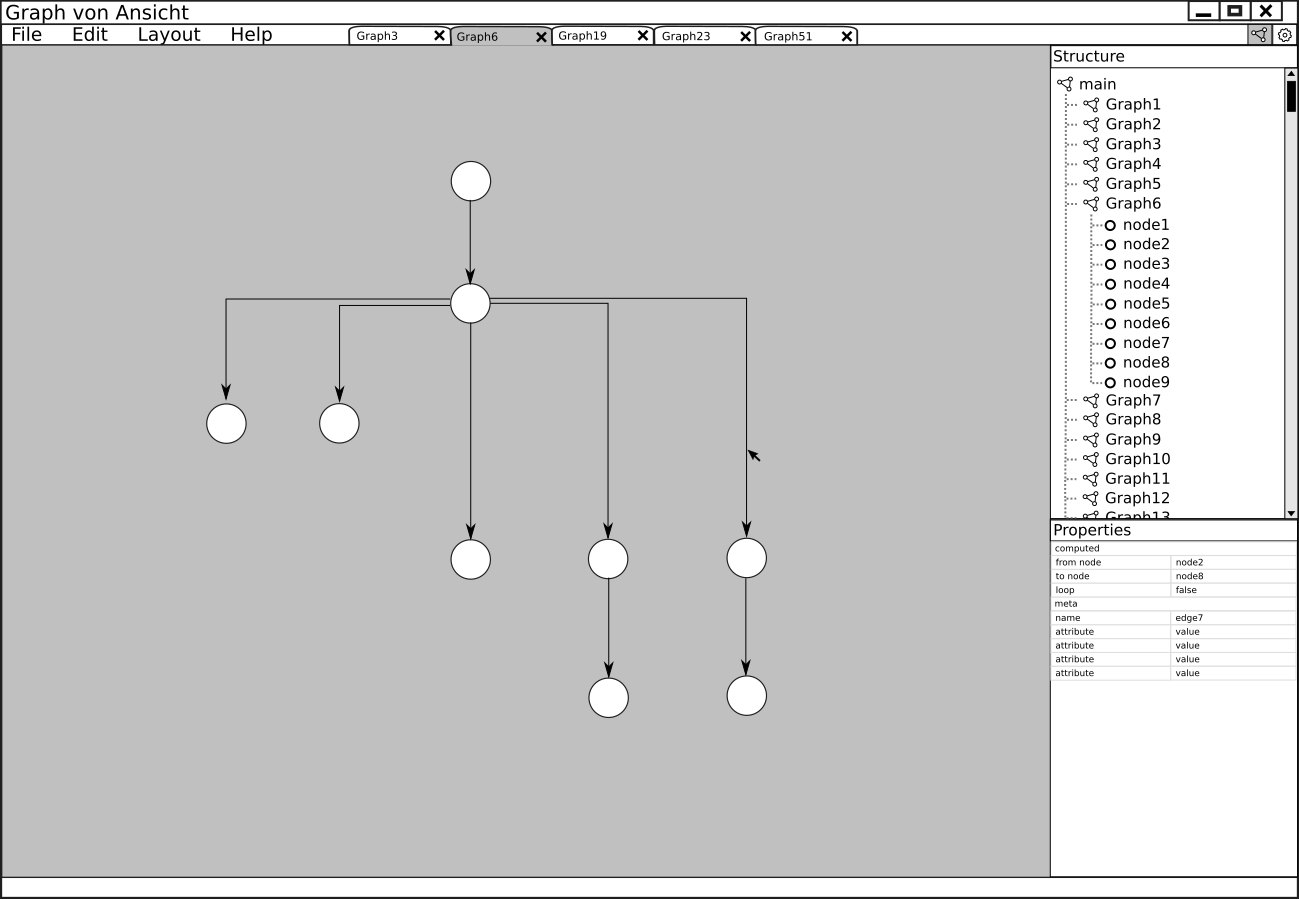
\includegraphics[width=380pt]{resourcen/gui_view_showInfoInProperties_edge.png}
  \caption{Eigenschaftenansicht von Ecken}
  \label{fig:gui_view_showInfoInProperties_edge}
\end{figure}

\begin{figure}[ht]
  \centering
  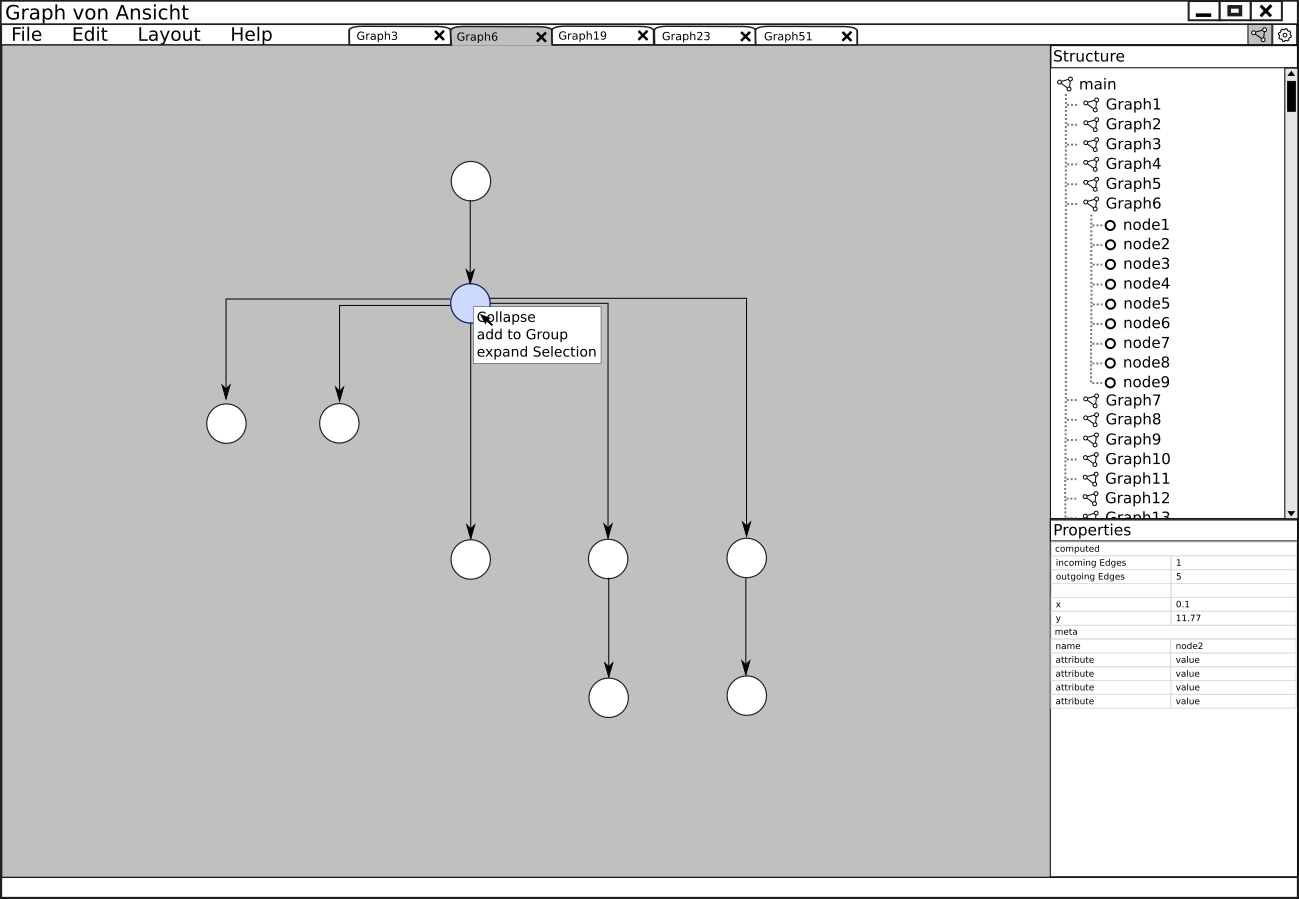
\includegraphics[width=380pt]{resourcen/gui_view_nodeMenu.png}
  \caption{Kontextmenü Knoten}
  \label{fig:gui_view_nodeMenu}
\end{figure}

\begin{figure}[ht]
  \centering
  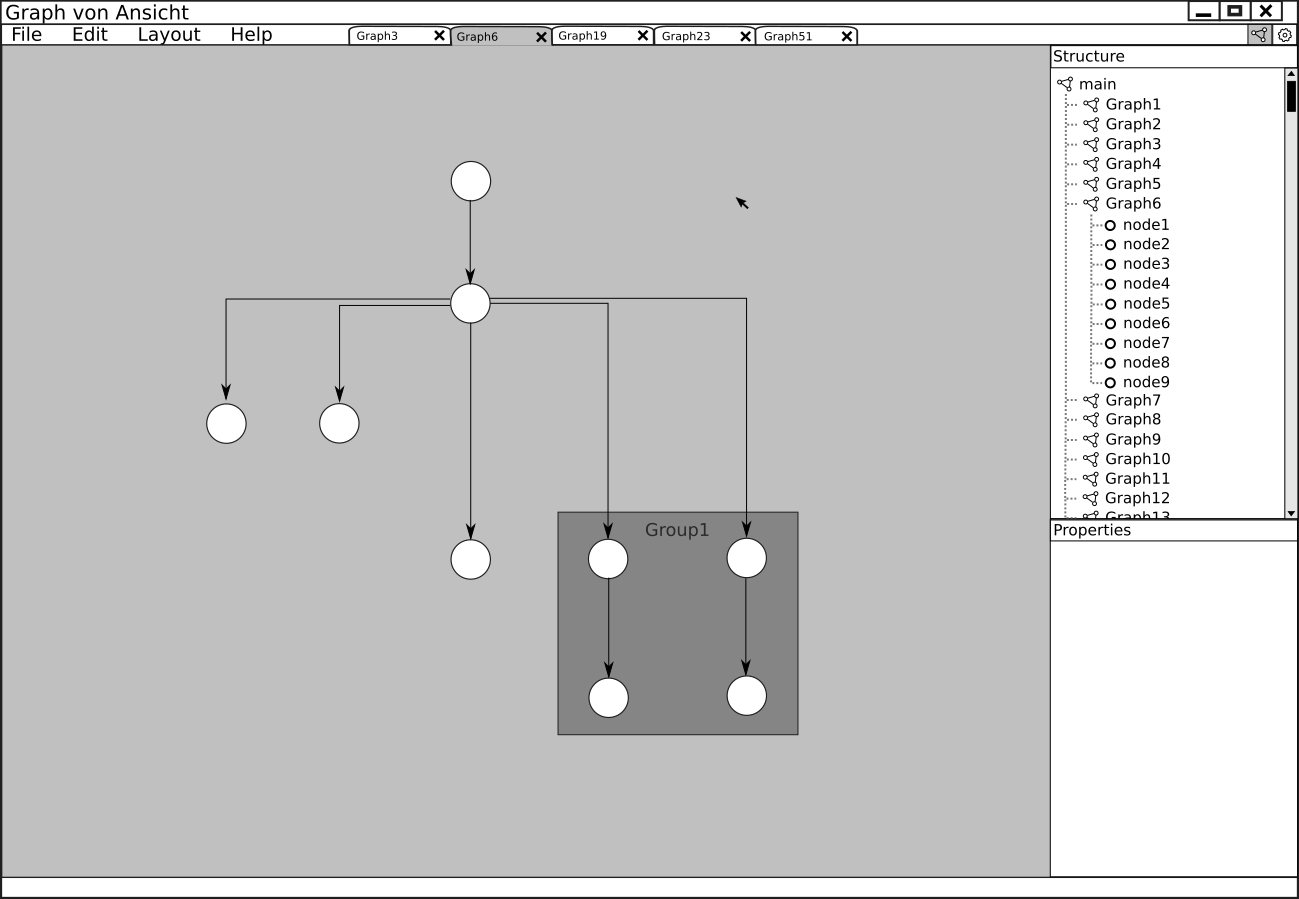
\includegraphics[width=380pt]{resourcen/gui_view_group.png}
  \caption{Gruppe von Knoten}
  \label{fig:gui_view_group}
\end{figure}

\begin{figure}[ht]
  \centering
  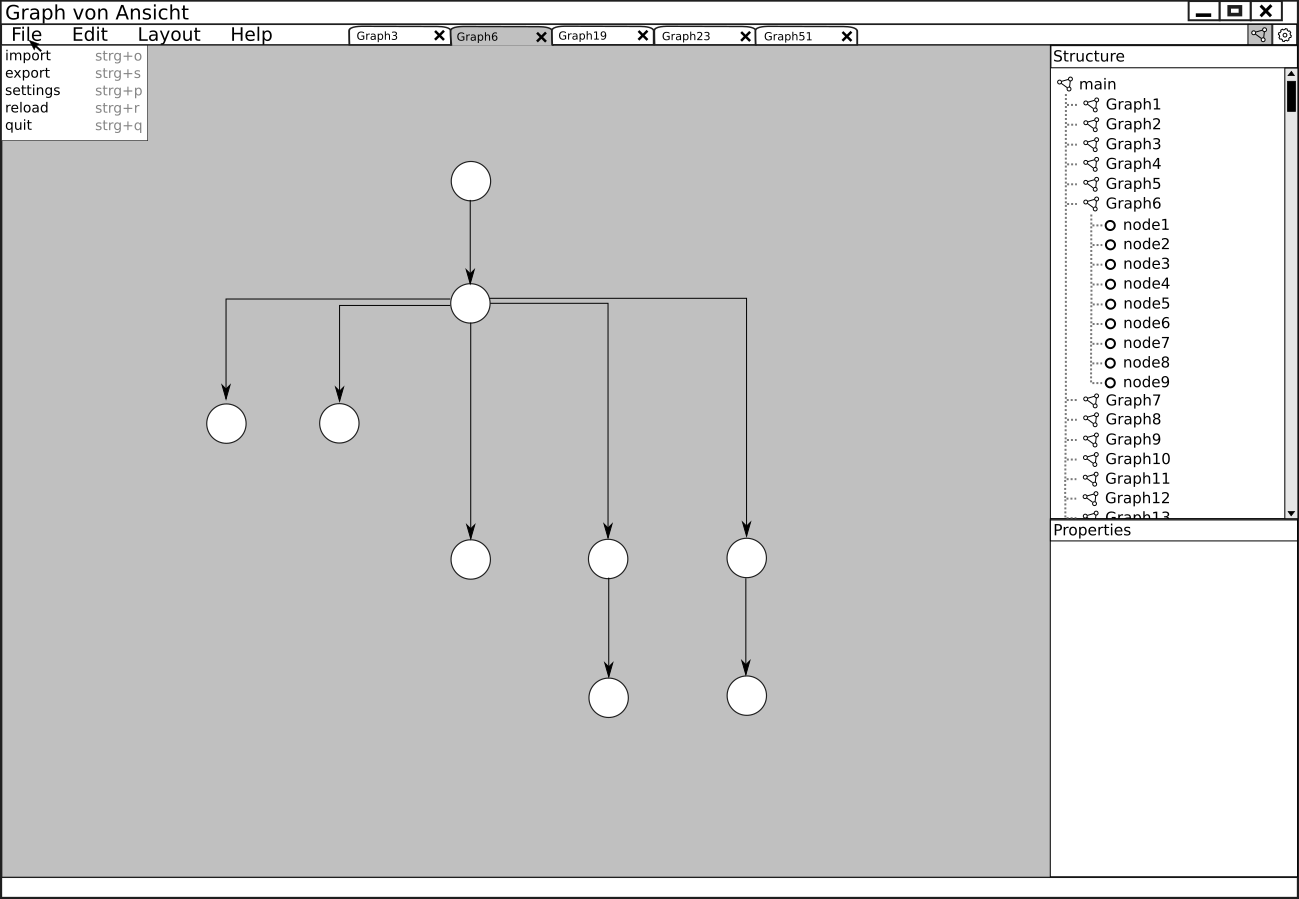
\includegraphics[width=380pt]{resourcen/gui_view_filemenu.png}
  \caption{Dateimenü}
  \label{fig:gui_view_filemenu}
\end{figure}

\begin{figure}[ht]
  \centering
  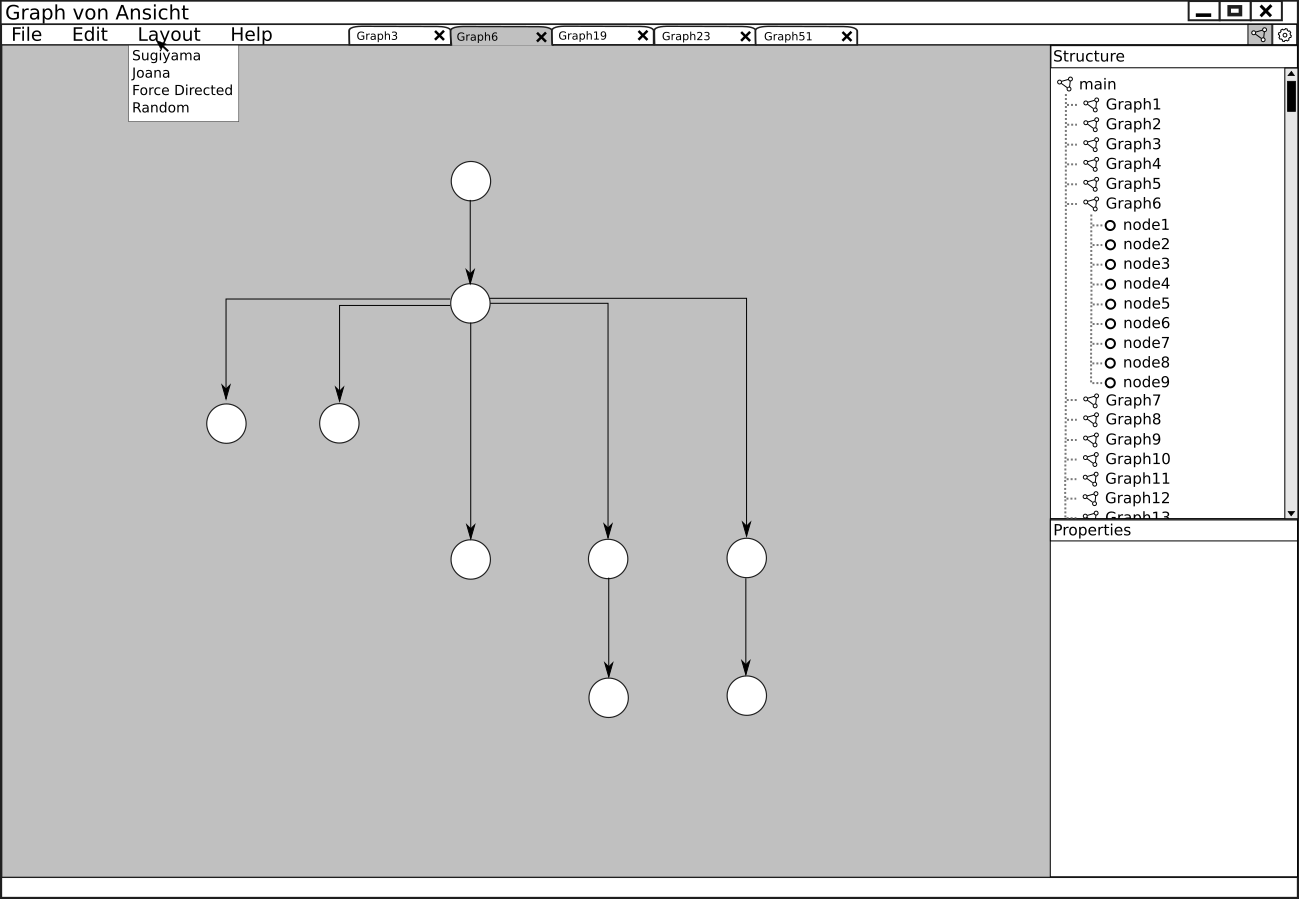
\includegraphics[width=380pt]{resourcen/gui_view_layoutmenu.png}
  \caption{Layoutmenü}
  \label{fig:gui_view_layoutmenu}
\end{figure}


\begin{figure}[ht]
  \centering
  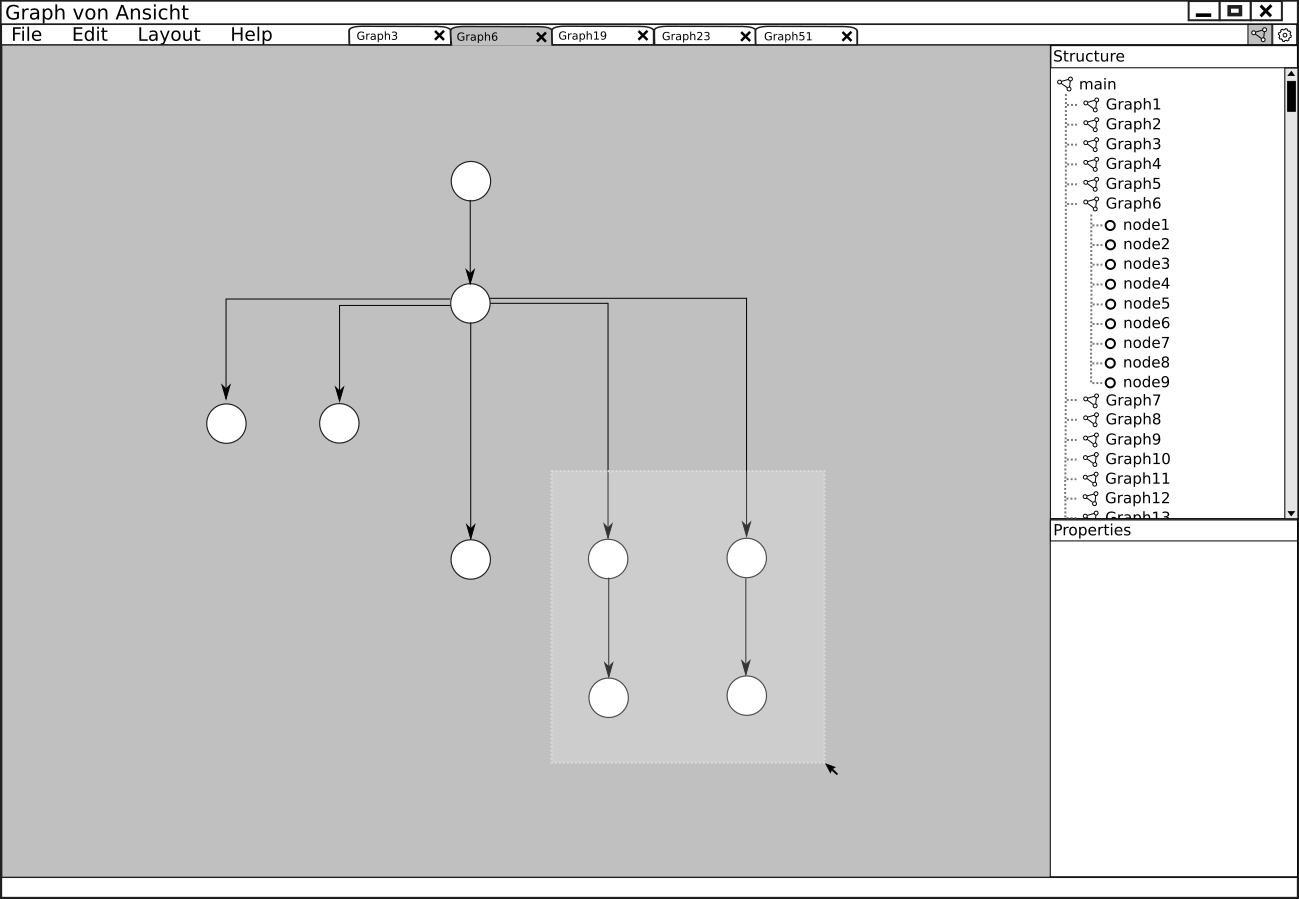
\includegraphics[width=380pt]{resourcen/gui_view_drawSelection.png}
  \caption{Auswahl mehrer Knoten und Kanten}
  \label{fig:gui_view_drawSelection}
\end{figure}

\begin{figure}[ht]
  \centering
  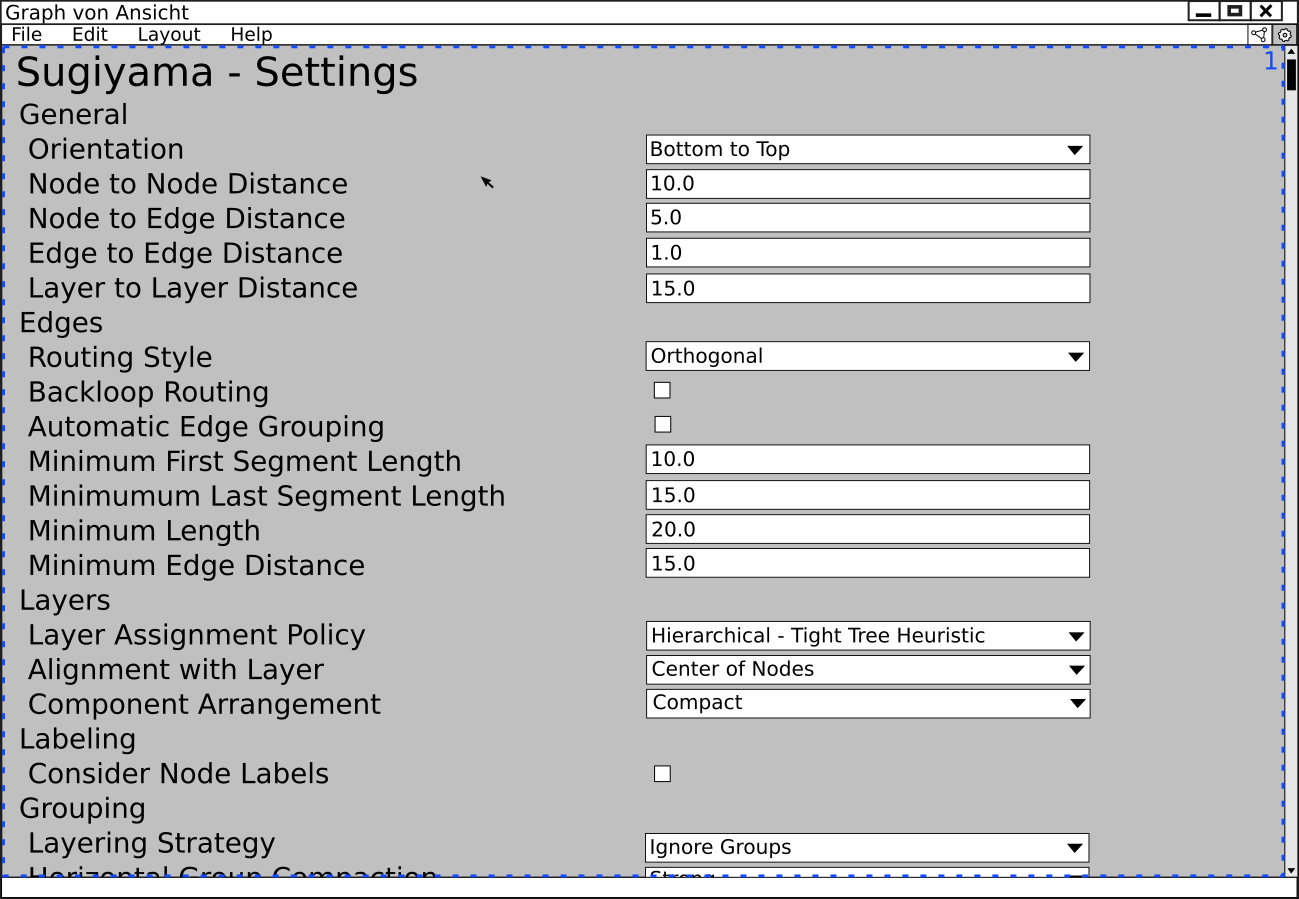
\includegraphics[width=380pt]{resourcen/gui_layoutsettings_settings.png}
  \caption{Einstellungen des Layoutalgorithmus}
  \label{fig:gui_layoutsettings_settings}
\end{figure}

\begin{figure}[ht]
  \centering
  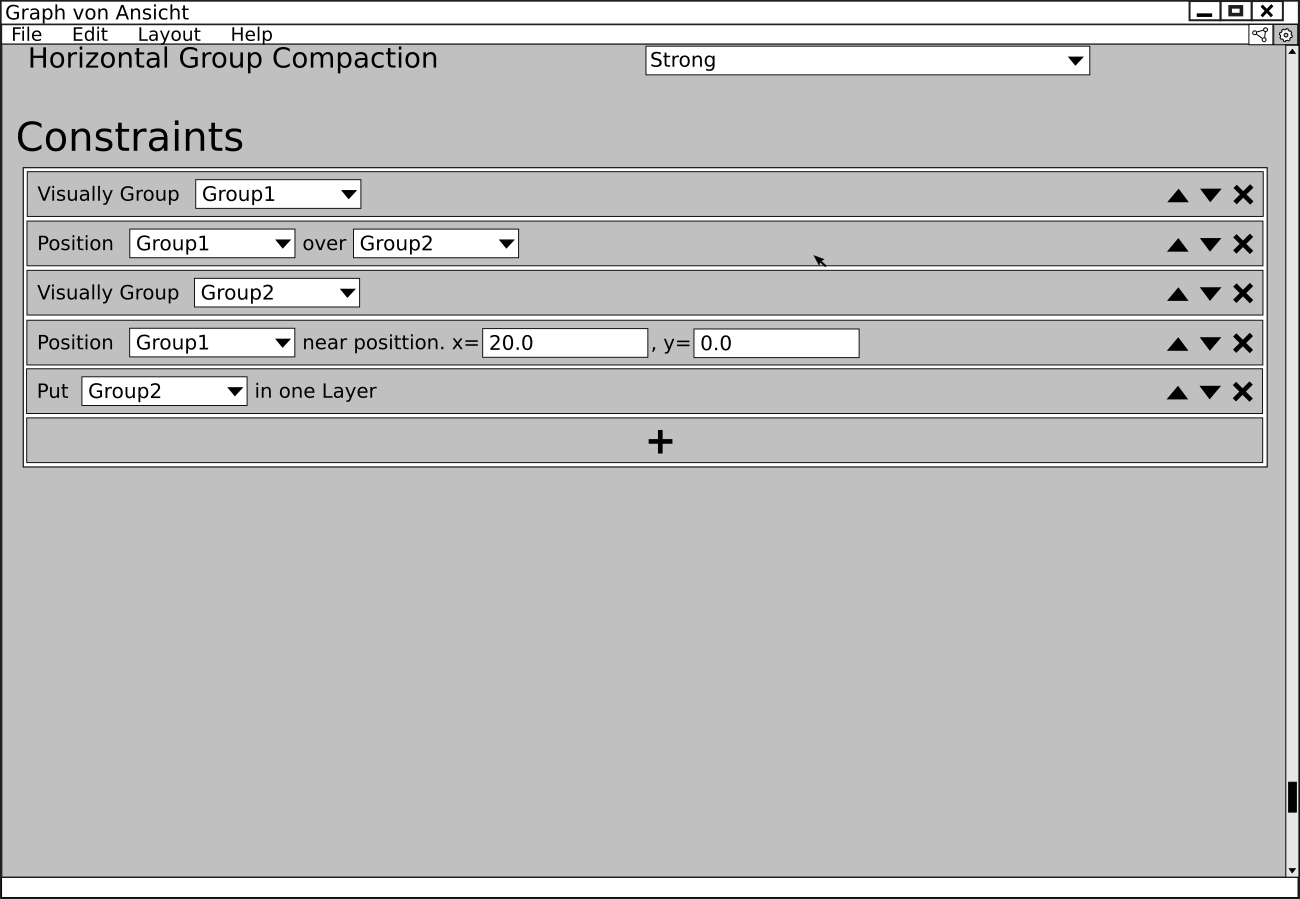
\includegraphics[width=380pt]{resourcen/gui_layoutsettings_constraints.png}
  \caption{Einstellungen der Layout Constraints}
  \label{fig:gui_layoutsettings_constraints}
\end{figure}

\begin{figure}[ht]
  \centering
  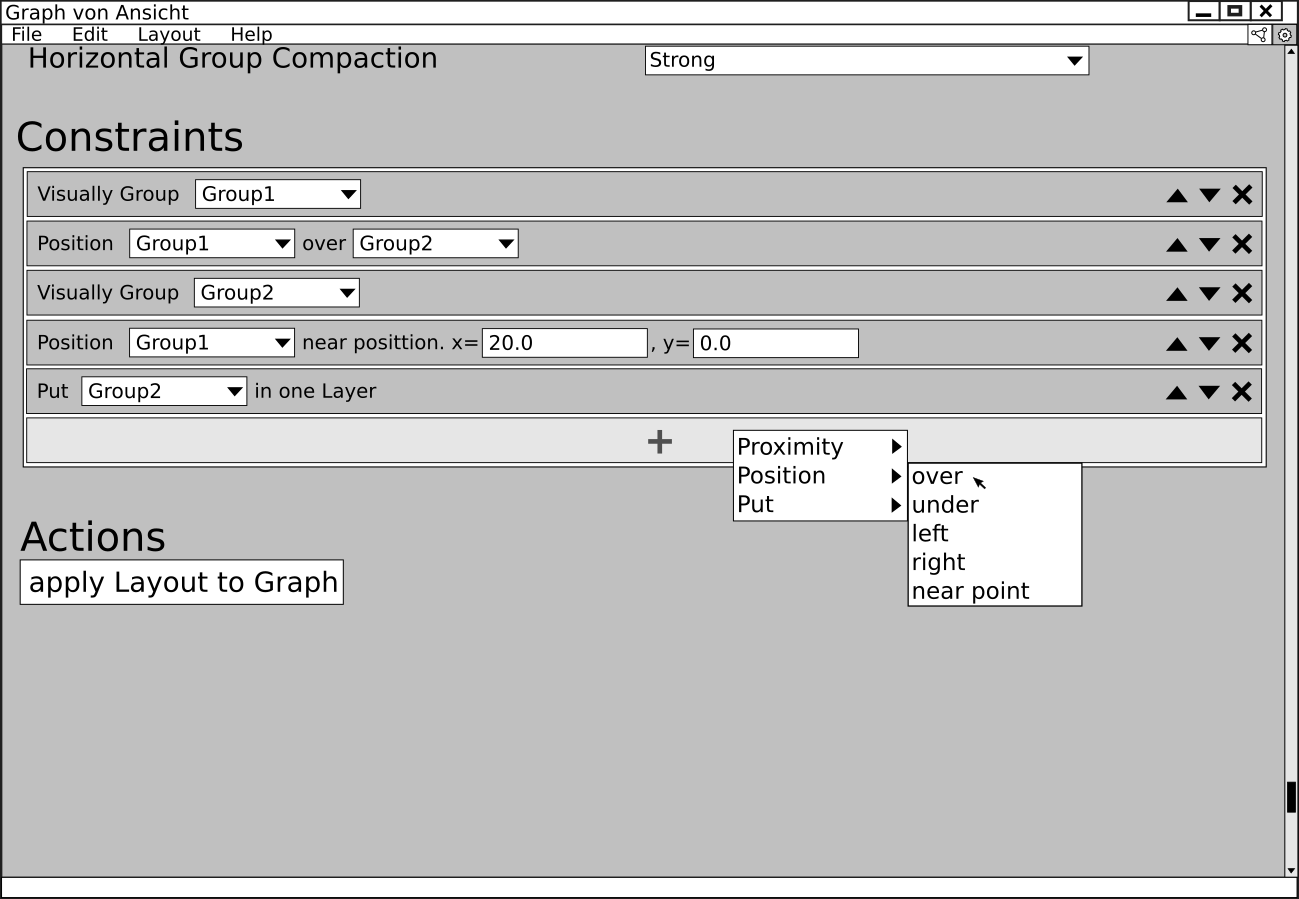
\includegraphics[width=380pt]{resourcen/gui_layoutsettings_constraints_new.png}
  \caption{neues Constraint hinzufügen}
  \label{fig:gui_layoutsettings_constraints_new}
\end{figure}

\begin{figure}[ht]
  \centering
  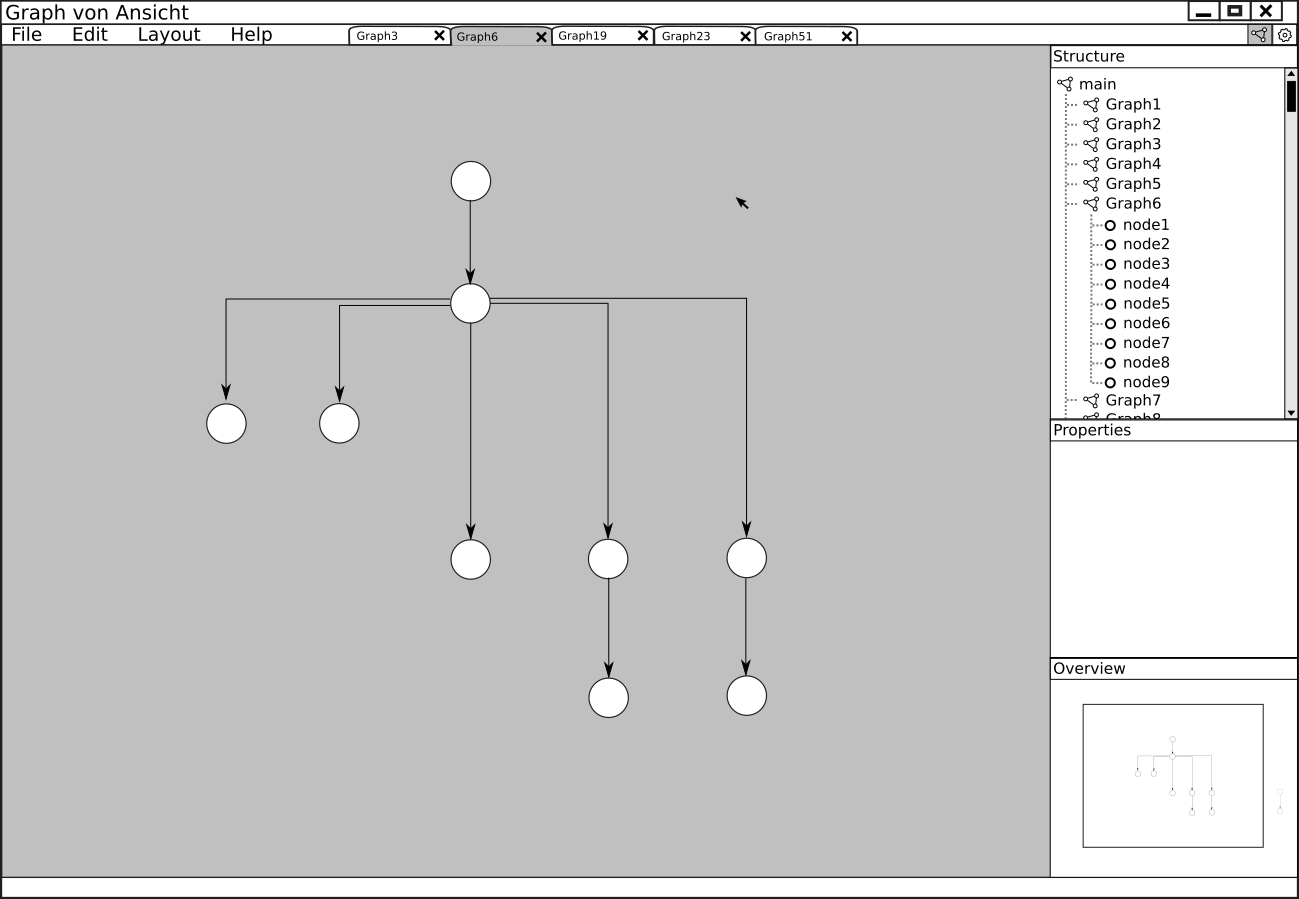
\includegraphics[width=380pt]{resourcen/gui_view_minimap.png}
  \caption{Übersichtsanzeige des aktuellen Graphen}
  \label{fig:gui_view_minimap}
\end{figure}

\begin{table}
  \caption{\gls{gui} Komponenten Referenzen}
  \begin{tabular}{lll}
    GUI Komponente & Abbildung & Referenznummer\\
    Graphansicht\label{gui:graphansicht} & \ref{fig:gui_view_treeview} & 1 \\
    Strukturansicht\label{gui:strukturansicht} & \ref{fig:gui_view_treeview} & 2 \\
    Tableiste\label{gui:tableiste} & \ref{fig:gui_view_treeview} & 3\\
    Menüleiste\label{gui:menuleiste} & \ref{fig:gui_view_treeview} & 4\\
    Hauptansicht(Fenster)\label{gui:hauptansicht} & \ref{fig:gui_view_treeview} & 5\\
    Informationsansicht\label{gui:informationsansicht} & \ref{fig:gui_view_showInfoInProperties_node} & 1 \\
    Einstellungen des Layoutalgorithmus\label{gui:layoutsetting} & a & b\\ %TODO: sinnvolle referenzen hinzufügen
  \end{tabular}
  \label{tab:guicomponents}
\end{table}